\chapter{Proposed Framework}
\label{ch:Framework}

In the \autoref{ch:FeatureExtraction} the features extraction process has been described. Before approaching the problem of performing \gls{nd} in \gls{glo:edge}, let's build a framework in \texttt{python} that runs on a \gls{pc} that is \emph{configurable}, \emph{modular}, \emph{expandable} and \emph{general purpose}. This framework will be used to test the features extraction process and to test the \gls{ml} algorithms before selecting one of them to be implemented in \gls{glo:edge} framework, which will be harder to configure.

A real case application would probably have several signals of several physical quantities, so a general approach that can manage different types of features, and extract from each of them the most relevant information, is needed.

The proposed framework is thought to be set up on any type and combination of sensors. The framework is thought to manage data that are correlated to a specific fault. For example, think about a \gls{cnc} machine like the one in \autoref{fig:cnc}. It has five axes, so a solution would be to instance the framework five times, one for each axis, linked to vibration sensors, temperature sensors etc. of the considered axis. This would allow us to pinpoint the fault to a specific axis. Another concern is, what if the single axis is seeing a normal condition, but the machine as a whole is not? This may happen if the tool has a problem: the vibration registered in the spindle would be normal in general, but would not be normal \emph{related} to the feed rate that another axis is imposing. To address this scenario, other instances of the framework can be set up, that also receive the speeds from the machine controller and the feed rate from the \gls{cnc} program as well as data from the sensors used in the other instances. This would allow us to detect a more complex fault, that is not characteristic of any part of the machine, but of the machine as a whole. The former kinds of instances would allow specific faults to be detected, giving also an idea of what the fault is, the latter would allow complex faults to be detected, but would not give a precise idea of what the fault is. The framework is thought to be able to manage both of these scenarios and to be able to manage them together.

\begin{figure}
  \centering
  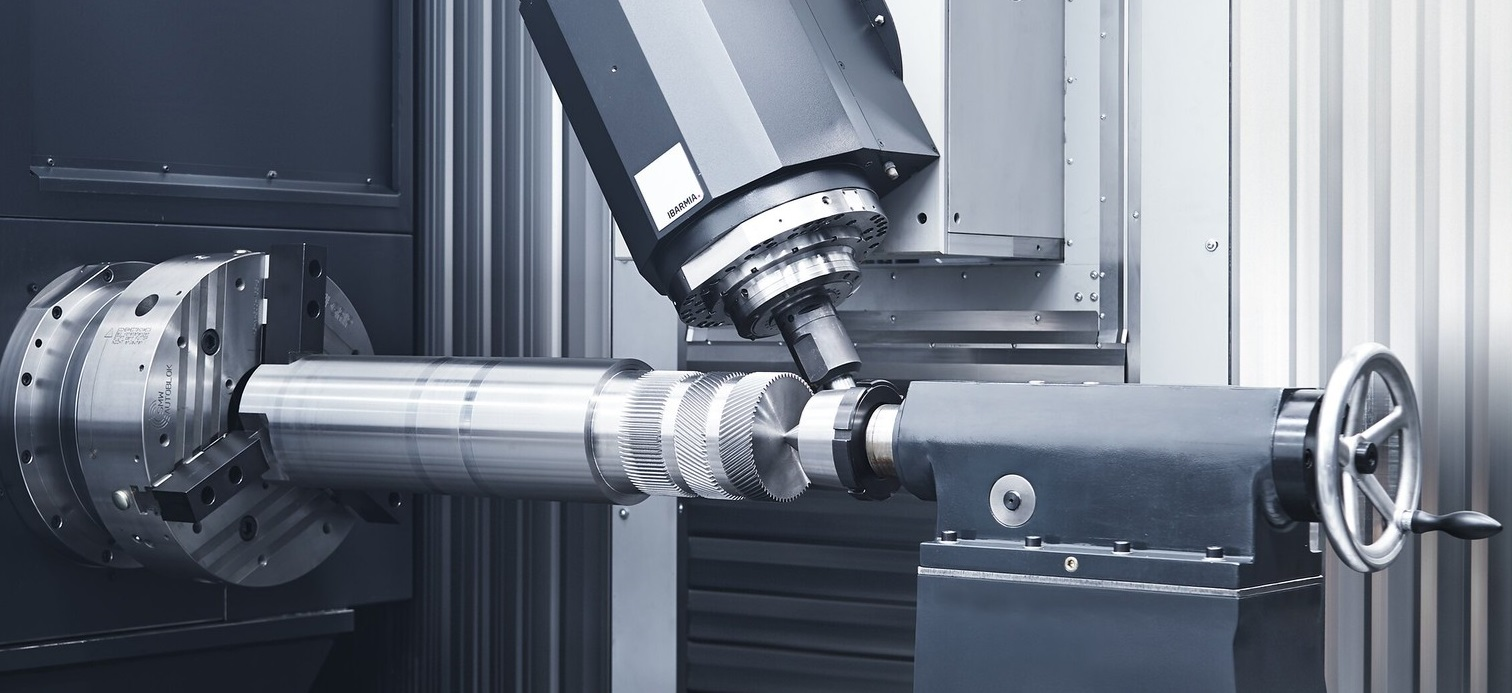
\includegraphics[width=.7\textwidth]{images/Framework/millmachine.jpg}
  \caption{A 5-axis \gls{cnc} milling machine. \cite{FagorAutomation}}
  \label{fig:cnc}
\end{figure}

\section{Commissioning}
\label{sec:commissioning}
To adapt the framework to a specific machine, the \gls{glo:commissioning} of the \gls{ml} system would have to be done in steps. Starting from the data acquisition and ending with the predictions of \gls{rul} and model updates, the steps are described in this section.

\subsection{Data structure}
\label{sec:Data_structure}
The first phase of adaptation of the framework to a machine is to define what data to sample and how to sample them. This includes the decision of which sensors to use, the sampling frequencies, the data acquisition system and which features are needed to be extracted from each sensor data. At this point, if more than one instance of the framework is needed, the sets of sensors and features to be used in each instance are defined. For example, in a shaft with two bearings, each with two accelerometers, the first instance of the framework would be linked to the first bearing, and would use the data from the two accelerometers to extract the features that are needed to detect the fault in the first bearing. The second instance of the framework would be linked to the second bearing, and would use the data from the other two accelerometers to extract the features that are needed to detect the fault in the second bearing. Optionally, a third instance of the framework would use the data from all four accelerometers to detect a generic fault in the shaft.
Those decisions influence the structure of the database, which will be described in \autoref{sec:Database}. 

\subsection{Data acquisition}
Once the structure of the data is defined, the first phase of the \gls{glo:commissioning} procedure is to set up the data acquisition. This has to be done when the machine is new or, at least, someone guarantees that the machine is in a healthy condition.

During the previous phase, the number of instances of the framework is defined. Each instance would have its own database. This phase is just a matter of storing the data that will be used to train the models the first time. A software agent, which we call \gls{glo:fieldagent} (\gls{fieldAg}), is responsible for this task. 
This phase lasts until the database is filled with enough data to train the models.

\subsection{Training}
The second phase of the \gls{glo:commissioning} procedure is to train the models. Once the healthy data are enough to characterize all the normal conditions of the maintained system, all the recorded data are elaborated by another software agent that we call \gls{glo:featAg} (\gls{fa}). This agent extracts all the features from the time-series and stores them in a structured way.

Once all the features are available in the database, another agent called \gls{glo:mla} (\gls{mla}) is responsible for training the models. All the models considered are \gls{uml} models. The models are trained on a standardized version of the feature matrix. The standardization is done \gls{wrt} the time evolution, \gls{ie} all the features used for training have a time evolution with zero mean and unit variance. This is done because most \gls{ml} algorithms are sensitive to the scale of the features.

All that has been said is valid for a single instance of the framework. If more than one instance is needed, the training phase has to be done for each instance.

\subsection{Evaluation}
At this point, a model that represents the normal condition of the system is available (actually a model for each instance of the framework). The next step is to evaluate the model.

In this phase, the machine continues to perform its normal operations. The \gls{glo:fieldagent} provides the sampled data, the \gls{glo:featAg} extracts the features and the \gls{glo:mla} evaluates the health of the system.
The proposed novelty/fault metric and procedure are specific to the model used, as described in the dedicated chapter about \gls{uml} models (\autoref{sec:clust_metric} for the k-means, \autoref{sec:dbscan_eval} for \gls{dbscan}, \autoref{sec:gauss_eval} for \gls{gmm}, \autoref{sec:svm_eval} for \gls{nu_svm}, \autoref{sec:iforest_eval} and \autoref{sec:lof_eval} for \gls{lof}). 

Now the \gls{nd} is up and running. The novelty metric is used to decide if the system is healthy or not. The metric is plotted for the user to see.
Note that in a classic \gls{ml} approach, the dataset is split into a training set and a test set. In this case, the test set is the data that are sampled during the evaluation phase. It's equivalent to saying that the model is trained on the past data and evaluated on the future data, or that the framework works in testing phase for an undetermined amount of time, until the user decides to update the models. This is equivalent to a test phase because if during this phase the framework outputs too many false positives, the user will decide to update the models. Otherwise, it means that the models are working properly and this phase can last indefinitely.

\subsection{Model update}
Once the metric overshoots the threshold, the \gls{mla} warns the user about the novelty detected, and starts to perform \gls{pdm} predicting the future evolution of the metric and the \gls{rul} of the system. 
Again, this condition can last indefinitely, once new data are sampled, the \gls{mla} evaluates the health of the system and updates the predictions.

It's up to the user to determine if the warning is a false positive, a novel but healthy behavior, or a real fault. In the first two cases, the user can decide to command the \gls{mla} to update the models. The snapshots that generated the warning are incorporated into the training set, and the models are retrained, returning to the evaluation phase. In the latter case, the user can simply perform the repairs/maintenance needed and restore the system to a healthy condition or can use the snapshots that generated the warning to train a new model that represents the fault condition.

If the user decides to train also the second model with the snapshot declared faulty, the system returns into the evaluation phase, but now the \gls{mla} outputs two metrics: one estimates the health of the system and the other how similar the behavior of the system is compared to any known fault condition.

\subsection{Predictions}
\label{sec:predictions}
\begin{figure}
    \centering
    \begin{subfigure}{\textwidth}
        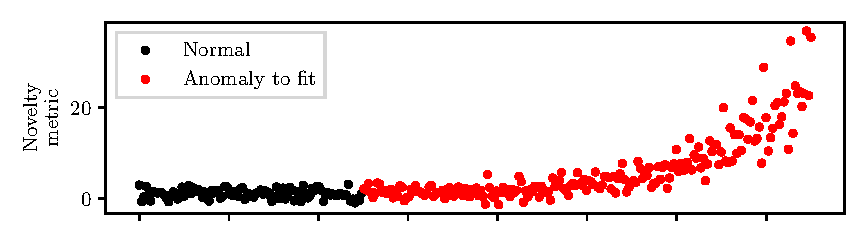
\includegraphics[width=\linewidth]{images/Framework/EXP_1.pdf}
        \caption{}
        \label{fig:exp_degradation_1}
    \end{subfigure}
    \begin{subfigure}{\textwidth}
        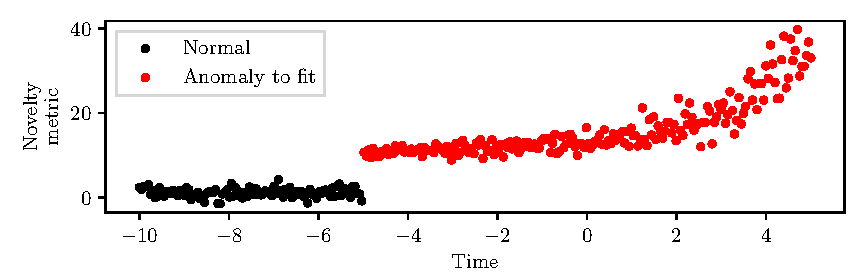
\includegraphics[width=\linewidth]{images/Framework/EXP_2.pdf}
        \caption{}
        \label{fig:exp_degradation_2}
    \end{subfigure}
    \caption{Novelty metric data to fit with an exponential curve.}
    \label{fig:mainfig}
    \label{fig:exp_degradation}
\end{figure}

The metric generated by the \gls{mla} is useful to detect novelties, with a \gls{cbm} approach. To actually perform \gls{pdm}, the \gls{mla} has also to predict the future evolution of the metric. Since, as anticipated in the introduction, this framework aims to output \emph{degradation based} predictions, a suitable fitting curve has to be used. Degradation-based failures are led by an initial defect that worsens over time. Often, the presence of an early defect further increases the worsening rate of the system. For this reason, and by observing the features evolution on publically available datasets, it seems reasonable to model the degradation with an exponential curve. This approach has been used in \cite{exp_degradation} and \cite{exp_degradation_NeuralNN}.

The candidate function to fit would then be:

\begin{equation}
    \label{eq:exp_degradation}
    f(t) = a \cdot e^{b \cdot t}
\end{equation}

where $a$ and $b$ are the parameters to be estimated. This may work in the case depicted in \autoref{fig:exp_degradation_1}, in which the novelty metric starts from zero and then increases exponentially. This is a problem for a general case in which the metric can have a plateau, or start as a step that signals the early defect, and then start an exponentially decay, as the example in \autoref{fig:exp_degradation_2}. In our case, in \autoref{ch:Unsupervised}, the set of defined metrics to be used are usually negative, to depict a normal behavior, and not zero. 

The \autoref{eq:exp_degradation} is nice, because by extracting the logarithm from both sides (and calling $y = \log(f(t))$) we obtain a linear equation that can be fitted easily with the least squares method described in \autoref{subsec:LS}, but for the reasons explained above, it's not suitable for our case. A better candidate is:

\begin{equation}
    \label{eq:exp_degradation_2}
    f(t) = a \cdot e^{b \cdot t} + c
\end{equation}

This is a better candidate because it can depict the case in which the metric starts from a value different from zero, and then increases exponentially.

\subsubsection{\texttt{Scipy} fit}
Unfortunately, \autoref{eq:exp_degradation_2} cannot be aranged in linear form, so the least squares solution has to be found with some other procedure. The \texttt{python} library \texttt{scipy.optimize} has a function called \texttt{curve\_fit} that can be used to fit a generic function to a dataset. The problem with this recursive solution is that is very sensitive to outliers and can't really estimate the parameter $c$ correctly, as is shown in \autoref{fig:exp_degradation_3}.

\subsubsection{Closed form fit with least squares}
Fortunately, in \cite{Exp_fit}, the author provides a \emph{nonrecursive} solution to the problem that minimizes the \gls{ls} error \gls{wrt} the parameters $a$, $b$ and $c$. The solution has been converted into the following \autoref{alg:expfit} and implemented in the framework. The fitting with this closed-form solution is shown in \autoref{fig:exp_degradation_3}. This optimal solution is used as default in the framework to predict the future evolution of the metric, the \texttt{scipy} implementation can still be used by changing a parameter in the configuration file because it has the advantage of fitting any function, so it may be useful in particular cases.

\begin{algorithm}
    \caption{Exponential regression of the novelty metric.}
    \label{alg:expfit}
    \begin{algorithmic}[1]
      \Function{ExpRegression}{$x, y$}
      \LineComment{$x = \{x_1, \dots, x_n\}$ is the array of x-coordinates of the data points.}
      \LineComment{$y = \{y_1, \dots, y_n\}$ is the array of y-coordinates of the data points.}
      \LineComment{Returns the parameters $a$, $b$ and $c$ of the exponential function $y(x) = a \cdot e^{b \cdot x} + c$ that minimize the least squares error.}
      \State $S_1 \gets 0$
      \State $S_k \gets S_{k-1}+\frac{1}{2}(y_k+y_{k-1})(x_k-x_{k-1}) \quad \text{for} \quad k \in [2, n]\cap \mathbb{N}$
      \State $\begin{bmatrix}
        A_1 \\
        B_1        
      \end{bmatrix} \gets \begin{bmatrix}
        \Sigma(x_k-x_1)^2 & \Sigma(x_k-x_1)\cdot S_k \\
        \Sigma(x_k-x_1)\cdot S_k & \Sigma S_k^2        
      \end{bmatrix}^{-1}
      \begin{bmatrix}
        \Sigma(y_k-y_1)(x_k-x_1) \\
        \Sigma(y_k-y_1)\cdot S_k  
      \end{bmatrix}$
      \State $a_1 \gets -\frac{A_1}{B_1}$
        \State $c_1 \gets B_1$
        \State $c_2 \gets c_1$
        \State $\theta_k \gets e^{c_2\cdot x_k} \quad \forall k \in [1, n]\cap \mathbb{N}$
        \State $\begin{bmatrix}
            a_2 \\
            b_2
        \end{bmatrix} \gets 
        \begin{bmatrix}
            n & \Sigma \theta_k \\
            \Sigma \theta_k & \Sigma \theta_k^2
        \end{bmatrix}^{-1}
        \begin{bmatrix}
            \Sigma y_k \\
            \Sigma y_k \cdot \theta_k
        \end{bmatrix}$
        \State $a \gets b_2$
        \State $b \gets c_2$
        \State $c \gets a_2$
        \State \Return $a, b, c$
      \EndFunction
    \end{algorithmic}
  \end{algorithm}
  

\begin{figure}
    \centering
    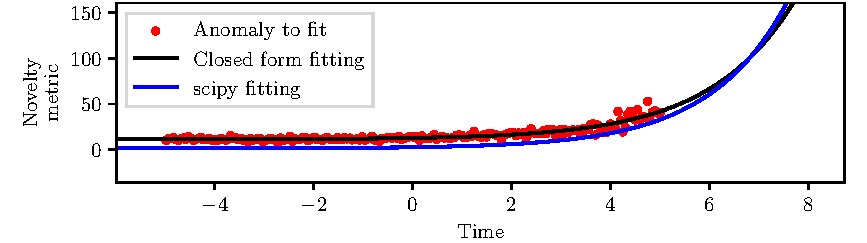
\includegraphics[width=\textwidth]{images/Framework/EXP_3.pdf}
    \caption{Fitted curve for \gls{rul} prediction. The \texttt{scipy} library fit fails to estimate the parameter $c$. The closed-form solution actually minimizes the error.}
    \label{fig:exp_degradation_3}
\end{figure}

\subsection{Instance structure}

\begin{figure}
    \centering
    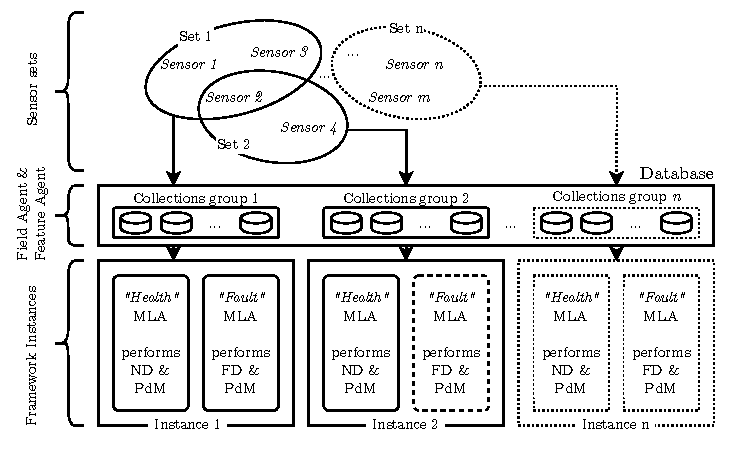
\includegraphics[scale=1]{images/Framework/FrameworkInstances.pdf}
    \caption{The structure of the instances of the framework.}
    \label{fig:instance_structure}
\end{figure}

As anticipated, in order to address different kinds of malfunctions, the framework is thought to be instanced several times on the same system. To visualize the structure of the instances, consider the general case described in \autoref{fig:instance_structure}. Any instance can rely on data gathered from any sensor subset and can perform \gls{nd} and \gls{fd}. In the figure, the first instance reads the first three sensors and has both the \gls{nd} and \gls{fd} algorithms active (this means that a fault dataset has been gathered in the past). The second instance reads a shared sensor with the first one, plus two new sensors. The dashed line surrounding the \gls{fd} algorithm means that is not active (no fault dataset has been gathered in the past, or it has not been trained). This instance performs only \gls{nd}. The last instance is just a general prosecution of the structure, that can be scaled indefinitely.


\section{Database}
\label{sec:Database}
In the previous \autoref{sec:commissioning}, the setup behaviour phases of the \gls{glo:frmwrk} have been described, referring to a generic \quoted{database}, without specifying the structure of the database. Let's now address the problem of storing the data efficiently and effectively. Instead of relying on \texttt{\gls{glo:python}} data structures, it is better to use a dedicated database manager.

The proposed \gls{glo:frmwrk} uses \gls{glo:mongodb} for the following reasons. It is a widely-used, open-source \gls{glo:nosql} database that is designed to handle unstructured or semi-structured data. It utilizes a document-oriented data model, storing data in flexible, \gls{json}-like \gls{bson} format. \gls{glo:mongodb} is suitable for implementation in a \gls{nd} \gls{glo:frmwrk} due to its scalability, flexibility, and real-time data processing capabilities. In novelty detection, the system often deals with diverse and dynamic data sources, making \gls{glo:mongodb}'s \quoted{unstructureness} advantageous for handling varying data formats and evolving data requirements. It has the ability to handle large volumes of data and support scaling allowing for efficient storage and retrieval of information in real-time, crucial for real-time applications. Moreover, \gls{glo:mongodb} has a rich query language and secondary indexes that allow for fast and efficient querying of data and a library for \texttt{\gls{glo:python}} that makes it easy to use.
The \gls{json} format is also human-readable, which makes it easy to understand the data stored in the database, and \quoted{mongoDB Compass} is a graphical user interface that allows one to easily explore the database.

\subsection{Collections}
\begin{longtblr}[
  caption = {Collections contained in the \gls{glo:mongodb} database},
  label = {tab:MongoDB_collections},
  ]{
  hline{1,11} = {-}{0.08em},
      hline{2} = {-}{},
    }
  \textbf{Collection} & \textbf{Content}                                       \\
  raw                 & time-series and information about them                 \\
  unconsumed          & \gls{glo:snap}s to be evaluated                              \\
  quarantined         & {\gls{glo:snap}s detected as novelty waiting to be declared  \\healthy, faulty or be discarded}\\
  healthy             & \gls{glo:snap} declared as normal behaviour                 \\
  healthy train       & {training dataset (scaled, processed, packet)          \\for the \gls{nd} \gls{uml} model}\\
  faulty              & \gls{glo:snap}s declared as faulty behaviour                 \\
  faulty train        & {training dataset (scaled, processed, packet)          \\for the \gls{nd} \gls{uml} model}\\
  models              & {models trained on healthy and faulty data the metrics \\and predictions to be shown}\\
  backup              & time-series, \gls{glo:feature}s, models, etc.
\end{longtblr}

\gls{glo:mongodb} structure is based on collections, which are groups of (\gls{json}) documents. A document is a set of key-value pairs that can be nested in several layers. Documents have a dynamic schema, which means that documents in the same collection do not need to have the same set of fields or structure, and common fields in a collection's documents may hold different types of data. To store the data needed by the \gls{glo:frmwrk} the collections reported in \autoref{tab:MongoDB_collections} are used.
In the following paragraphs, the structure and purposes of each collection are described.

\paragraph{Raw}
Thinking about the data flow, the first interface between the hardware and the software would be the sensor readings. Every sensor should have a name and be sampled at a constant frequency (or, at least, the sensors that provide data for frequency-domain \gls{glo:feature} extraction should have a constant sampling frequency). This data is stored in the {raw} collection, with the \gls{json} structure summarized in \autoref{tab:raw_json},
where \texttt{\textunderscore id} is the unique identifier of the document, \texttt{timestamp} is the time at which the data was acquired, in \gls{iso} format, and \texttt{Sensor 1} to \texttt{Sensor n} are the names of the sensors. 

\begin{longtable}{lll}
  \caption{Structure of the \quoted{raw} collection \gls{json} configuration file.}\label{tab:raw_json}\\ 
  \toprule
  \textbf{Field} & \textbf{Sub-Field} & \textbf{Type} \endfirsthead 
  \hline
  \texttt{\textunderscore}id &  & string \\
  timestamp &  & \gls{iso} date \\*
  \multirow{2}{*}{sensor 1} & sampling frequency & float \\*
   & time-serie & list[float] \\*
  \multirow{2}{*}{sensor 2} & sampling frequency & float \\*
   & time-serie & list[float] \\
  $\dots$ & $\dots$ & $\dots$ \\*
  \multirow{2}{*}{sensor~$n$} & sampling frequency & float \\*
   & time-serie & list[float] \\
  \bottomrule
  \end{longtable}

  Each sensor has a \texttt{sampFreq} field that contains the sampling frequency of that particular sensor, and a \texttt{timeSerie} field that contains the data acquired by the sensor, as a list. The \texttt{timeSerie} field is a list of floating point numbers, that can be of any length. Note that the sampling frequencies of different sensors can be different, for example, if a timestamp contains $1\si{\s}$ period of data, a vibration sensor would be linked to an array with several thousands of samples, while a temperature sensor would be linked to only one sample.
  
\paragraph{Unconsumed}
Once defined the structure that the time-series will have in the database, let's define the structure of the \gls{glo:snap}s. The \gls{glo:feature}s extracted from the time-series are stored in the {unconsumed} collection, with the \gls{json} structure described in \autoref{tab:unconsumed_json}.

\begin{longtable}{lll}
  \caption{Structure of the \quoted{unconsumed} collection \gls{json} configuration file.}\label{tab:unconsumed_json}\\ 
  \toprule
  \textbf{Field} & \textbf{Sub-Field} & \textbf{Type} \endfirsthead 
  \hline
  \texttt{\textunderscore}id & - & string \\
  timestamp & - & \gls{iso} date \\
  \vcell{sensor 1} & \vcell{mean} & \vcell{float} \\*[-\rowheight]
  \printcelltop & \printcellmiddle & \printcellmiddle \\
   & root mean square & float \\
   & peak to peak & float \\
   & standard deviation & float \\
   & skewness & float \\
   & kurtosis & float \\
   & wavelet coefficient~$1$ & float \\
   & wavelet coefficient~$2$ ~ & float \\
   & $\vdots$ & $\vdots$ \\
   & wavelet coefficient~$2^{\text{three dept}}$ & float \\
  sensor 2 & mean & float \\
   & root mean square & float \\
   & peak to peak & float \\
   & standard deviation & float \\
   & skewness & float \\
   & kurtosis & float \\
   & wavelet coefficient~$1$ & float \\
   & wavelet coefficient~$2$ & float \\
   & $\vdots$ & $\vdots$ \\
   & wavelet coefficient~ $2^{\text{three dept}}$~~ & float \\
  $\vdots$ & $\vdots$ & $\vdots$ \\
  sensor~$n$ & mean & float \\
   & root mean square & float \\
   & $\vdots$ & $\vdots$ \\
   & wavelet coefficient~ ~~$2^{\text{three dept}}$ & float \\
  novelty evaluated flag & - & boolean \\
  \bottomrule
  \end{longtable}
  
Notice that different sensors can have different \gls{glo:feature}s. The \quoted{novelty evaluated} field is a boolean that is set to \texttt{false} when the \gls{glo:snap} is created, and is set to \texttt{true} when the \gls{nd} algorithm evaluates the \gls{glo:snap}. This field is used to avoid evaluating the same \gls{glo:snap} multiple times while leaving it in the collection until also the \gls{fd} algorithm is performed. At this point, the \gls{glo:snap} will be moved either to the backup collection, discarded or to the quarantine collection if either the \gls{nd} or the \gls{fd} flag it.

\paragraph{Quarantined}
The \quoted{quarantined} collection is used to store the \gls{glo:snap}s that were flagged as \quoted{novelty} by the \gls{nd} algorithm or as \quoted{faulty} by the \gls{fd} algorithm (or were flagged by both of them). The structure is the same as the \quoted{unconsumed} collection, but the \quoted{novelty evaluated} field is not present since, at this point, the \gls{glo:snap}s are guaranteed to have been evaluated. The \gls{glo:snap}s in this collection are waiting to be declared as \quoted{healthy} or \quoted{faulty} by the user or to be discarded.

\paragraph{Healthy}
The idea behind the \quoted{healthy} collection is to store the \gls{glo:snap}s that are acquired during the first work phase of the \gls{glo:frmwrk}, before training, or the \gls{glo:snap}s that were in the \quoted{quarantine} collection and were declared as healthy by the user. The documents in this collection have the same structure as the documents in the \quoted{quarantined} collection.

\paragraph{Healthy train}
In this collection the healthy \gls{glo:snap}s are packed together in different documents, each of them useful in a different phase of the training process.

{The first document has the \texttt{id} \texttt{training\textunderscore set}, that contains all the \texttt{N} training \gls{glo:snap}s, each of them with \texttt{n} sensors signals, characterized by \texttt{F} \gls{glo:feature}s. For ease of accessibility, every bottom-nested field is a list of \texttt{N} elements. The structure is resumed in \autoref{tab:train_json}.}


\begin{longtable}{lll}
\caption{Structure of the \quoted{healthy train} collection \gls{json} configuration file.}\label{tab:train_json}\\ 
\toprule
\textbf{Field} & \textbf{Sub-Field} & \textbf{Type} \endfirsthead 
\hline
\texttt{\textunderscore}id & - & string \\
timestamp & - & list[\gls{iso} date] \\
\vcell{sensor 1} & \vcell{\gls{glo:feature} 1} & \vcell{list[float]} \\*[-\rowheight]
\printcelltop & \printcellmiddle & \printcellmiddle \\
 & \gls{glo:feature} 2 & list[float] \\
 & $\vdots$ & $\vdots$ \\
 & \gls{glo:feature} F & list[float] \\
sensor 2 & \gls{glo:feature} 1 & list[float] \\
 & \gls{glo:feature} 2 & list[float] \\
 & $\vdots$ & $\vdots$ \\
 & \gls{glo:feature} F & llist[loat] \\
$\vdots$ & $\vdots$ & $\vdots$ \\
sensor~$n$ & \gls{glo:feature} 1 & list[float] \\
 & \gls{glo:feature} 2 & llist[loat] \\
 & $\vdots$ & $\vdots$ \\
 & \begin{tabular}[c]{@{}l@{}}\gls{glo:feature} F\\\end{tabular} & list[float] \\
\bottomrule
\end{longtable}


This collection contains other three documents:
\begin{itemize}
  \item \texttt{training set scaled}, that contains the scaled training set, having the same structure as the \texttt{training set} document;
  \item \texttt{training set MIN MAX}, that contains the minimum and maximum values of the \gls{glo:feature}s of the training set, useful to plot the \gls{glo:feature}s with a reference of the bounds of the training set. It has the same structure of the \texttt{training set} document, but the bottom-nested fields are lists of two elements (the minimum and the maximum value);
  \item \texttt{StandardScaler\textunderscore pickled}. It contains the \texttt{StandardScaler} object that was used to scale the training set. This object is encoded in \gls{glo:pickle}, and it is used during the evaluation phase to scale the \gls{glo:snap}s before evaluating them.
\end{itemize}

\paragraph{Faulty}
This collection serves the same exact purpose as the \quoted{healthy} collection, but for the faulty \gls{glo:snap}s. Faulty \gls{glo:snap}s are not discarded because they can be used to train the \gls{fd} \gls{uml} algorithm.

\paragraph{Faulty train}
This collection serves the same exact purpose as the \quoted{healthy train} collection, but for the faulty \gls{glo:snap}s.

\paragraph{Models}
This collection contains the models trained on the healthy and faulty data and a buffer of the predictions and metrics to be displayed to the user.

The structure of the models' documents is just an identifier and the \texttt{\gls{glo:python}} object of the model, encoded in \gls{glo:pickle}. The structure of the predictions and metrics documents is the \autoref{tab:model_json}:

\begin{longtable}{lll}
  \caption{Structure of the \quoted{models} collection \gls{json} configuration file.}\label{tab:model_json}\\ 
  \toprule
  \textbf{Field} & \textbf{Sub-Field} & \textbf{Type} \endfirsthead 
  \hline
  \texttt{\textunderscore}id & - & string \\
  timestamp & - & list[\gls{iso} date] \\
  values & - & list[float] \\
  assigned \gls{glo:clust} & - & list[int] \\
  anomaly flag & - & list[bool] \\
  prediction curve parameters & - & pickle format \\
  \bottomrule
  \end{longtable}

\paragraph{Backup}
The backup collection is a general-purpose container for any document that needs to be stored for backup purposes. It can contain time-series, \gls{glo:feature}s, models, etc. The structure of the documents in this collection is the same as the structure of the documents in the other collections.


\section{Software Agents}
\label{sec:agents}

\begin{figure}
    \centering
    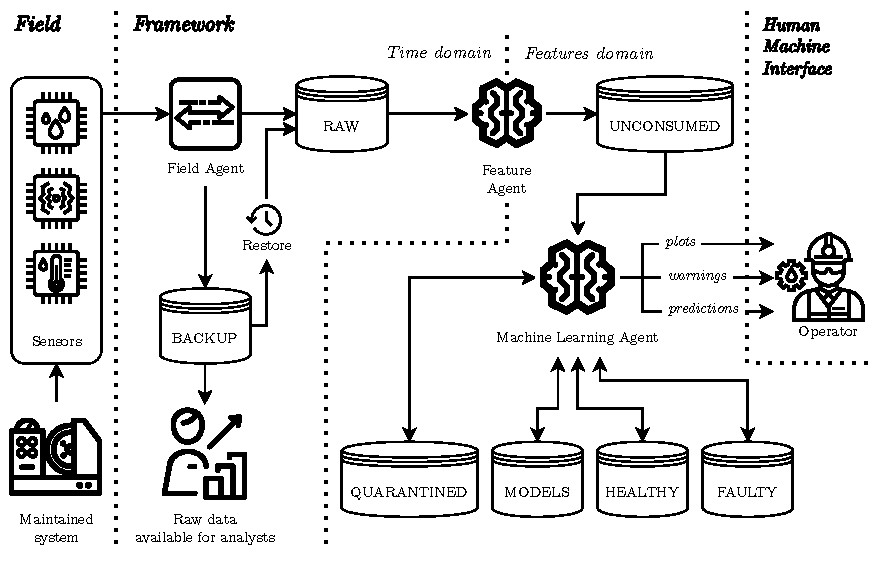
\includegraphics[width=\textwidth]{images/Framework/Framework_structure.pdf}
    \caption{Framework logical structure}
    \label{fig:Framework_structure}
\end{figure}

In the previous sections, the software agents were mentioned as the main actors in the framework. This section will provide a more detailed description of the software agents, their role and their interaction with the environment and the data, following the flow from the hardware through the time-series, the feature domain to the \gls{ml} algorithms. The reference layout is the one in \autoref{fig:Framework_structure}. 

Software \gls{glo:agent}s are autonomous programs that perform a specific task in a cycle. In \texttt{python}, the agents are classes that are instanced and run in a loop.

\subsection{Field Agent}
\label{subsec:FieldAgent}
\begin{figure}
    \centering
    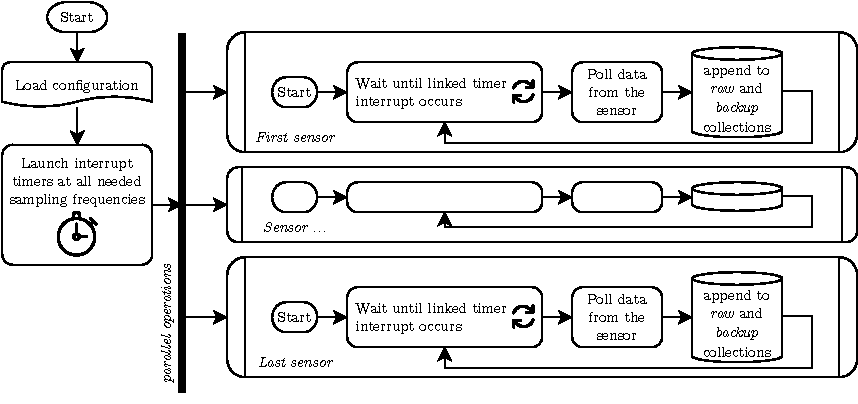
\includegraphics[scale=1]{images/Framework/Field_Agent_flowchart.pdf}
    \caption{Field Agent flowchart}
    \label{fig:Field_Agent_flowchart}
\end{figure}

This is the interface between the hardware and the software. It is responsible for the acquisition of the data from the sensors and the communication with the database. Since some features will be related to the spectrum of the data, a precise and fixed sampling frequency is needed. Hence, the \gls{fieldAg} must incorporate a synchronization with the \gls{adc}. It stores data in the \emph{raw} collection and the \emph{backup} collection. In \autoref{fig:Field_Agent_flowchart}, the flow of operations are shown as a flowchart, emphasizing the importance of the synchronization with the \gls{adc}. This software agent has not been implemented in \texttt{python}, because the experimental validation of this work, as it will be described in \autoref{sec:Validation}, has been performed directly on the \gls{glo:edge} platform. During the tests on the publicly available datasets, an abstract version of the \gls{fieldAg} has been used, that reads the data from the \gls{csv} files.


\subsection{Feature Agent (FA)}
\label{subsec:FeatureAgent}
\begin{figure}
    \centering
    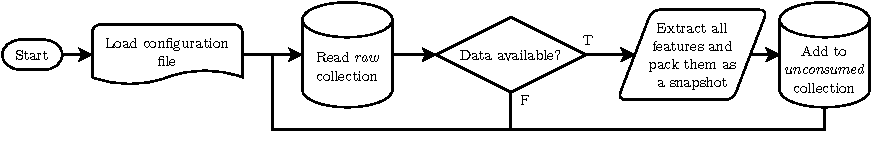
\includegraphics[width=\textwidth]{images/Framework/FA_flowchart.pdf}
    \caption{Feature Agent flowchart}
    \label{fig:FA_flowchart}
\end{figure}

The \gls{fa} is responsible for the feature extraction from the raw data. It reads the data from the \emph{raw} collection, extracts the features and stores them in the \emph{unconsumed} collection. The flow of operation is shown in \autoref{fig:FA_flowchart}. The \gls{fa} is implemented in \texttt{python} and it is a class that has been designed to be easily expandable and configurable. The methods implemented in the \gls{fa} class are shown in \autoref{tab:FA_methods}.


\begin{longtable}{p{0.4\textwidth}p{0.5\textwidth}}
    \caption{\gls{fa} class implemented methods\label{tab:FA_methods}}\\ 
    \toprule
    \textbf{Method} & \textbf{Description} \endfirsthead
    \hline
    readFromRaw & reads a snapshot from the raw collection and stores it in the instance self \\
    extractFeatures & extract all the features from the current snapshots, for all the sensors \\
    extractTimeFeautures & extract~mean,~rms, P2P, std, skewness and kurtosis, based on the config file for the specified sensor \\
    extractFreqFeautures & extract the wavelet coefficients for the specified sensor, up to the configured depth \\
    deleteFromraw & delete current snap record from the \emph{raw} collection \\
    writeToUnconsumed & write the extracted features to the \emph{unconsumed} collection \\
    initialize\_barPlotFeatures & initializes the bar plot of the features that is shown to the user \\
    barPlotFeatures & updates the bar plot with new features \\
    run & perform the agent operations in loop. idle until new data are available in \emph{raw} collection \\
    \bottomrule
\end{longtable}
    

\subsection{Machine Learning Agent (MLA)}
\label{subsec:MLA}
The \gls{mla} is responsible for the training and the evaluation of the \gls{ml} models. It reads the data from the \emph{unconsumed} collection, evaluates the snapshot and stores the result in the \emph{models} collection, it also constantly updates the information about the novelty or fault metric to the user. The flow of operation is shown in \autoref{fig:MLA_structure}. The methods implemented in the \gls{mla} class are shown in \autoref{tab:MLA_methods}.

This agent is designed to be configured as a \gls{nd} or \gls{fd} agent with just one hyperparameter. If it is instanced for \gls{nd}, it uses the healthy collection as a training dataset, if it is instanced for \gls{fd} it uses the faulty collection. The metric used to evaluate the snapshots is the novelty metric for \gls{nd} and the fault metric for \gls{fd}. According to the procedure defined in \autoref{alg:eval_new_snapshot}.

\begin{figure}[htbp]
    \centering
    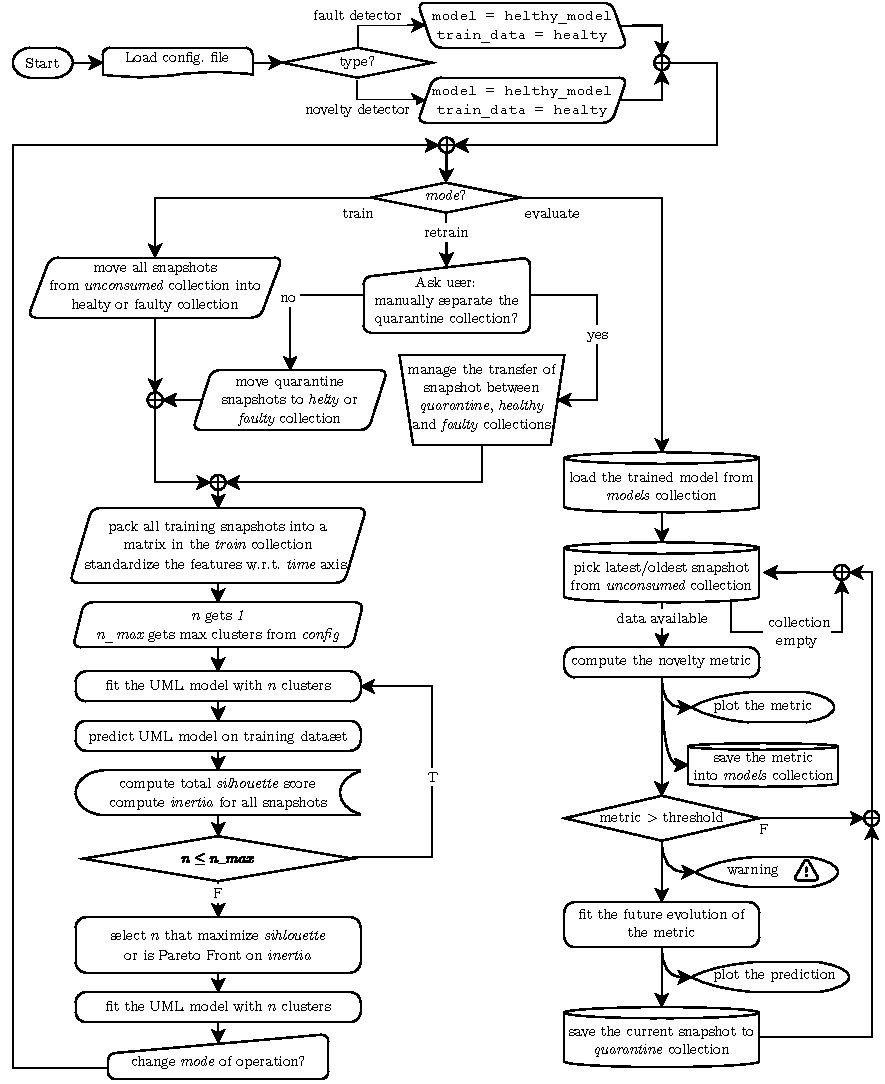
\includegraphics[width=\textwidth]{images/Framework/MLA.pdf}
    \caption{Machine Learning Agent flowchart. When it is instanced for \gls{nd}, the \gls{mla} uses the healthy collection as a training dataset, when it is instanced for \gls{fd} it uses the faulty collection.}
    \label{fig:MLA_structure}
\end{figure}


\begin{longtable}{p{0.4\textwidth}p{0.5\textwidth}}
    \caption{\gls{mla} class implemented methods\label{tab:MLA_methods}}\\ 
    \toprule
    \textbf{Method} & \textbf{Description} \endfirsthead 
    \hline
    run & run the \gls{mla} according to its current state \\
    evaluate & evaluate the current snapshot based on the novelty or the fault metric, according to the type of instance \\
    predict & fit the novelty metric with a degradation curve to predict the future evolution~ \\
    mark\_snap\_evaluated & set the evaluated flag to true for the current snapshot \\
    delete\_evaluated\_snap & remove the evaluated snapshots from the \emph{unconsumed} collection \\
    scale\_features & scales the features of the current snapshot according to the standard scaler used during the training procedure \\
    evaluate\_error & compute the novelty or fault metric for the current snapshot, according to the type of instance \\
    calculate\_train\_cluster\_dist & compute the radiuses of the clusters during the training procedure \\
    prepare\_train\_data & performs the preprocessing of the data before training the model \\
    pack\_train\_data & pack the training snapshot in a matrix \\
    \_\_move\_to\_train & move an entire collection of snapshots to the training collection \\
    standardize\_features & make all the features in the training matrix have zero mean and unitary variance \\
    save\_features\_limits & save the unscaled bounds of the training features \\
    save\_StdScaler & store the standard scaler instance in \gls{glo:pickle} into the database \\
    retrieve\_StdScaler & restore the standard scaler instance in \gls{glo:pickle} from the database \\
    save\_KMeans & store the model instance in \gls{glo:pickle}  \\
    retrieve\_KMeans & restore the model instance in \gls{glo:pickle}  \\
    \_append\_features & append the current features in a document \\
    train & performs the training of the clustering models \\
    evaluate\_silhouette & compute the silhouette score of the training set snapshots \\
    \_\_plot\_silhouette & plots the silhouette score against the number of clusters \\
    evaluate\_inertia & compute the inertia score of the training set snapshots \\
    \_\_plot\_inertia & plots the inertia score against the number of clusters \\
    packFeaturesMatrix & format all the training features as a matrix \\
    retrain & perform a new training of the models \\
    \bottomrule
    \end{longtable}
    
\newpage
\subsection{Configuration of the framework}
All the configurations described in this chapter are stored in the \texttt{config.yaml} file. This file is read by the agents at the beginning of their execution. The configuration file is divided into sections by topic: database, models etc. An example of a valid configuration file for the \gls{ims} dataset is shown in \autoref{lst:configyaml}.
\begin{minted}[
    gobble=4,
    frame=single,
    linenos,
    breaklines
  ]{yaml}
    Database:           # Database configuration
    URI:                mongodb://localhost:27017   # MongoDB URI
    db:                 Shaft                       # Database name
    collection:       # Collection configuration
      back:             BACKUP                      # Backup collection name
      raw:              RAW                         # Raw data collection name
      unconsumed:       UNCONSUMED                  # Unconsumed data collection name
      healthy:          HEALTHY                     # Healthy data collection name
      healthy_train:    HEALTHY_TRAIN               # Healthy data collection name for training (some healthy data are not used if not novelty)
      quarantined:      QUARANTINED                 # Quarantined data collection name
      faulty:           FAULTY                      # Faulty data collection name
      faulty_train:     FAULTY_TRAIN                # Faulty data collection name for training (some faulty data are not used if not fault novelty)
      models:           MODELS                      # Models collection name
    sensors:          # Expected sensors in the database
      Bearing 1 x:    # Sensor 1 name
        features:     # Features configuration
          wavPowers:    on                          # Wavelet powers
          mean:         on                          # Mean value
          rms:          on                          # Root mean square
          peak:         on                          # Peak to peak value
          std:          on                          # Standard deviation
          skew:         on                          # Skewness
          kurt:         on                          # Kurtosis
      Bearing 1 y:    # Sensor 2 name
        features:     # Features configuration
          wavPowers:    on                          # Wavelet powers
          mean:         on                          # Mean value
          rms:          on                          # Root mean square
          peak:         on                          # Peak to peak value
          std:          on                          # Standard deviation
          skew:         on                          # Skewness
          kurt:         on                          # Kurtosis
      ...:
      Bearing 4 y:    # Sensor n name
        features:     # Features configuration
          wavPowers:    on                          # Wavelet powers
          mean:         on                          # Mean value
          rms:          on                          # Root mean square
          peak:         on                          # Peak to peak value
          std:          on                          # Standard deviation
          skew:         on                          # Skewness
          kurt:         on                          # Kurtosis
  wavelet:           # Wavelet packet transform configuration
    type:               db10                        # Type of wavelet to use
    mode:               symmetric                   # Mode of the packet transform
    maxlevel:           6                           # Max level -> num of features = 2^level
  kmeans:            # kmean configuration
    max_clusters:       100                         # Max number of clusters
    max_iterations:     1000                        # Max number of iterations
    error_queue_size:   1                           # number of predictions parameters to keep in queue for plotting/predicting
    error_plot_size:    2000                        # Size of the plotting queue
  
  novelty:           # Novelty/fault configuration
    threshold:          0.10                        # Threshold for novelty / fault detection: relative percentage of the distance to the cluster w.r.t the max distance to the assigned cluster in the training set
    forecast_threshold: 0.8                         # Threshold for novelty / fault prediction
    n_fit:              250                         # Number of samples used to fit the prediction curve
    outlier_filter:     1                           # Number of consecutive outliers to filter (1 means two outliers will be considered as novelty/fault)
    regressor:          exp                         # Regressor to use for prediction: exp, scipy, poly. if exp uses a custom function, if scipy uses scipy.optimize.curve_fit, if poly fit polynomial of degree
  
  miscellanea:
    logpath:            C:\Users\JohnSmith\Documents\framework  # Path to the logs
\end{minted}

\subsection{Command Line Interface (CLI)}
\label{subsec:CLI}
\begin{figure}[h!]
    \centering
    \includegraphics[width=\textwidth]{images/Framework/cli.png}
    \caption{Command Line Interface help message}
    \label{fig:cli}
\end{figure}

To ease the interaction with the user, a \gls{cli} has been implemented. It relies on the \texttt{click} and \texttt{typer} libraries for \texttt{python}. The \gls{cli} allows the user to instance the agents, to configure the framework, to monitor the agents and to interact with the database. All the commands are provided with a help message that can be accessed by typing \texttt{--help} after the command, as shown in \autoref{fig:cli} for the command \texttt{run-machine-learning-agent}.
The commands implemented in the \gls{cli} are shown in \autoref{tab:CLI_commands}.



\begin{longtable}{p{0.4\textwidth}p{0.5\textwidth}}
    \caption{\gls{cli} implemented commands\label{tab:CLI_commands}}\\ 
    \toprule
    \textbf{Command} & \textbf{Description} \endfirsthead 
    \hline
    copy-collection            &Move all the documents from one collection to another\\
    create-empty-db            &Create an empty database in MongoDB. The database should not exist already. It is configured according with "config.yaml" file.\\
    ims-converter              &Transfer the data from the gls{ims} textual files into the MongoDB database in a suitable way.\\
    fault-indicator            &This function plots the fault metric.\\
    novelty-indicator          &This function plots the novelty metric.\\
    move-collection            &Move all the documents from one collection to another\\
    plot-features              &Plot the features of the last snapshot in the UNCONSUMED collection\\
    run-feature-agent          &Run the Feature Agent - takes the last snapshot from RAW collection, extracts features and writes them to UNCONSUMED collection\\
    run-machine-learning-agent &Run the Machine Learning Agent \\
    \bottomrule
    \end{longtable}